% ================================================================ 5.3
% SERL (keep screenshots, add SAC lineage)
\begin{frame}{Robotic RL in Practice: SERL}
\vfill
\centering
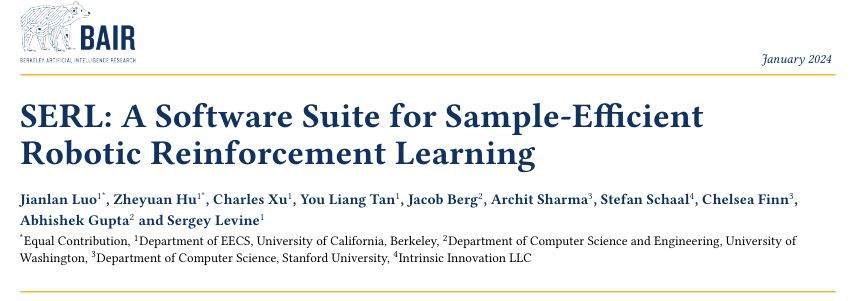
\includegraphics[width=0.9\linewidth,keepaspectratio]{images/rl-real-world/figures/serl-title.jpg}%
\srcnote{\scriptsize Luo et al. \href{https://serl-robot.github.io/}{SERL: A Software Suite for Sample-Efficient Robotic Reinforcement Learning}, 2024.}
\vfill
\end{frame}

\begin{frame}{SERL}
\begin{itemize}\itemsep0.4em
    \item A software framework for sample-efficient RL on real robots: an
          off-policy deep RL method plus tooling for computing rewards, resetting
          the environment, and a high-quality controller for a widely-adopted arm.
    \item \empr{SAC lineage:} \textbf{SERL $\leftarrow$ RLPD $\leftarrow$ SAC}, the same maximum-entropy method you already know, now learning on real
          hardware in \emph{minutes}.
\end{itemize}
\vfill
\centering
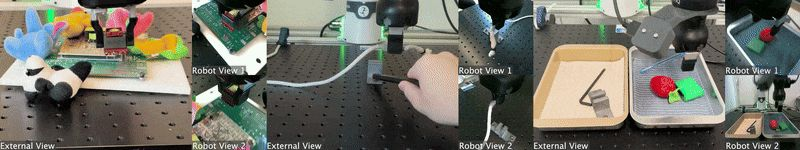
\includegraphics[width=0.92\linewidth,keepaspectratio]{images/rl-real-world/figures/robot-filmstrip.jpg}%
\srcnote{\scriptsize \href{https://github.com/rail-berkeley/serl}{github.com/rail-berkeley/serl}}
\end{frame}

\begin{frame}{SERL: Results}
\vfill
\centering
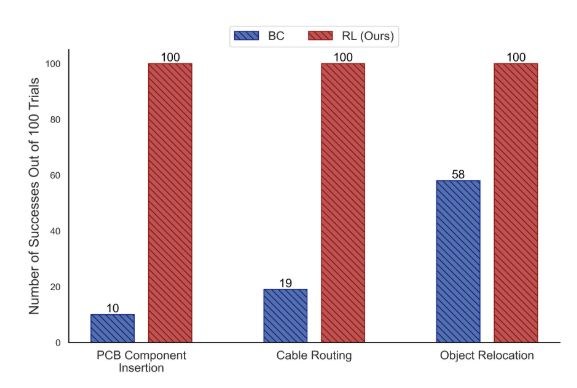
\includegraphics[width=0.6\linewidth,height=0.78\textheight,keepaspectratio]{images/rl-real-world/figures/robot-results.jpg}
\vfill
\end{frame}
